\underline{Ferromagnetyzm}

Oddziaływania magnetyczne dipoli w ferromagnetykach dążą do ustawienia ich równolegle. Zależą więc od ich wzajemnego ustawienia, ale nie wyróżniają żadnego bezwzględnego kierunku w przestrzeni. Są symetryczne względem obrotów w zwykłej przestrzeni konfiguracyjnej. Powyżej pewnej temperatury, zwanej temperaturą Curie ($ T_C $), energia kinetyczna dipoli jest na tyle duża, że nie pozwala na ich wzajemną korelację. Stan ferromagnetyka wykazuje więc też symetrię obrotową. Jeżeli temperatura spadnie poniżej $ T_C $, to oddziaływania dipoli są już na tyle silne, że porządkują ustawienie dipoli i ferromagnetyk ma pewne namagnesowanie wyróżniające jakiś kierunek w przestrzeni. Powyżej $ T_C $ wszystkie kierunki były takie same, żaden nie był wyróżniony, poniżej $ T_C $ ferromagnetyk "spontanicznie" wybiera jakiś kierunek magnetyzacji. Zwróćmy uwagę na to, że oddziaływanie dipoli nie ulega zmianie, dalej ma symetrię obrotową. W tym sensie teoria nadal jest symetryczna. To stan ferromagnetyka nie wykazuje symetrii. Zjawisko to można symulować, korzystając z modelu Isinga (patrz zagadnienie wyżej).

\underline{Model żerowania mrówek}

Mrówki mają do dyspozycji dwie ścieżki między mrowiskiem, a pokarmem. Prawdopodobieństwo wyboru ścieżki $ i $:\newline
$ \dfrac{(x_i + k)^{\alpha}}{(x_i + k)^{\alpha} + (x_j + k)^{\alpha}} $, gdzie:\newline
$ x_i $ - ilość feromonu na ścieżce $ i $,\newline
$ \alpha $ - stopień nieliniowości wyboru,\newline
$ k $ - stopień atrakcyjności ścieżki bez feromonu (im większy tym tym więcej feromonu potrzeba do preferencji danej ścieżki).

Dodatkowe założenia:
\begin{itemize}
	\item Stała liczba mrówek $ \varphi $.
	\item Mrówki wracają tą samą drogą, co przyszły.
	\item Ilości feromonu pozostawionego na ścieżce zależy od jej długości lub od jej jakości $ q_i $.
	\item Feromon ulatnia się ze stałą prędkością $ v $.
\end{itemize}

Tempo zmian koncentracji feromonu:\newline
$ \dfrac{dx_1}{dt} = \varphi q_1 \dfrac{(x_1 + k)^{\alpha}}{(x_1 + k)^{\alpha} + (x_2 + k)^{\alpha}} - vx_1 $,\newline
$ \dfrac{dx_2}{dt} = \varphi q_2 \dfrac{(x_2 + k)^{\alpha}}{(x_1 + k)^{\alpha} + (x_2 + k)^{\alpha}} - vx_2 $

Rozważmy rozwiązanie równowagowe dla dwóch jednakowych ścieżek: $ q_1 = q_2 = q $ oraz $ \dfrac{dx_1}{dt} = \dfrac{dx_2}{dt} = 0 $:\newline
$ vx_1 = \varphi q p_1 $,\newline
$ vx_2 = \varphi q p_2 $,\newline
$ \dfrac{x_1}{p_1} = \dfrac{x_2}{p_2} \rightarrow \bigg( \dfrac{x_2 + k}{x_1 + k} \bigg)^{\alpha} = \dfrac{x_2}{x_1} $

W przypadku możliwości wyboru między wieloma celami, załamanie symetrii zachodzi, gdy opłacalnym jest dla większości grupy, by podejmować tą samą decyzję (rys.~\ref{ants1}).

\begin{figure} [H]
	\centering
	\begin{subfigure}{.95\textwidth}
		\centering
		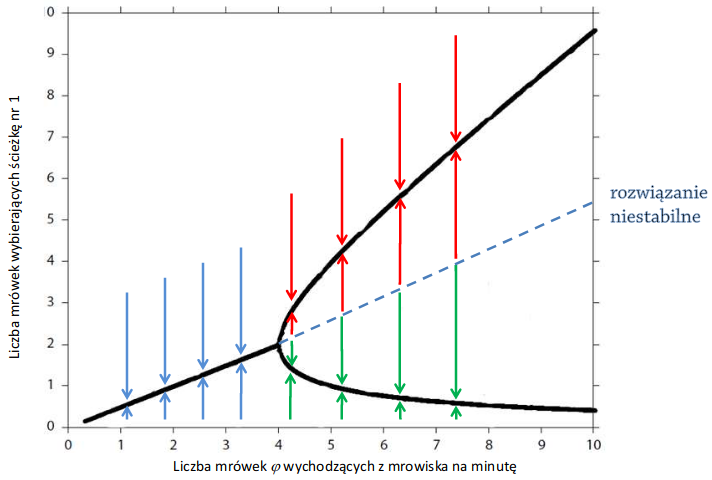
\includegraphics[width=1.0\linewidth]{EDMIIssues/Figures/ants1.png}
	\end{subfigure}
	\caption{Diagram bifurkacyjny dla $ q = v = 1 $, $ k = 2 $.}
	\label{ants1}
\end{figure}

Dla różnych wartości $ q_i $ rozwiązanie łamiące symetrię jest niestabilne (rys.~\ref{ants2})

\begin{figure} [H]
	\centering
	\begin{subfigure}{.95\textwidth}
		\centering
		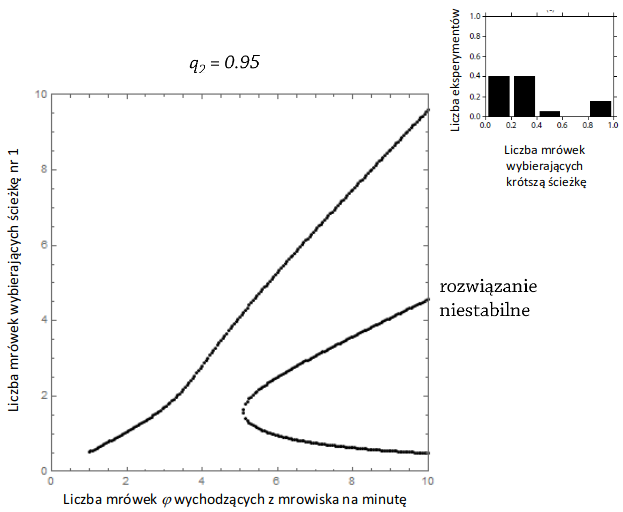
\includegraphics[width=1.0\linewidth]{EDMIIssues/Figures/ants2.png}
	\end{subfigure}
	\caption{Diagram bifurkacyjny dla $ q_1 = v = 1 $, $ k = 2 $.}
	\label{ants2}
\end{figure}